The number of roots of the polynomial, $s^{7}+s^{6}+7 s^{5}+14 s^{4}+31s^{3}+73 s^{2}+25 s+$ $200,$ in the open left half of the complex plane is

(A) 3

(B) 4

(C) 5

(D) 6\\
We will be using the concept of Routh-Hurwitz Criterion.\\
\textbf{Routh-Hurwitz Criterion:} The number of roots of the polynomial that are in the right half-plane is equal to
the number of sign changes in the first column.

\begin{itemize}
    \item Routh–Hurwitz stability criterion is a mathematical test that is a necessary and sufficient condition for the stability of a linear time invariant control system.
\end{itemize}

Rules for generating Routh-Hurwitz Table.

\begin{enumerate}
    \item Label the rows of Routh table from highest power to the lowest power.
    \item List alternative coefficients starting with the highest order coefficients in the first row.
    \item List alternative coefficients starting with the next highest order coefficients in the second row.
    \item Each entry is the negative of determinant of the previous two entries in the previous two rows divided by the entry in the first column directly above the row.
    \item The left hand column of the determinant is always the first column of the previous two rows.
    \item The right hand column is the elements of the column above and to the right.
    \item The table is complete when all of the rows are completed down to $s^0$.
\end{enumerate}
The Routh-Hurwitz Table for given equation $s^{7}+s^{6}+7 s^{5}+14 s^{4}+31s^{3}+73 s^{2}+25 s+$ $200,$ is calculated as follows

\begin{center}

\begin{tabular}{ |p{1.25cm}|p{1.25cm}|p{1.25cm}|p{1.25cm}|p{1.25cm}|  }
\hline
$s^7$ & 1 & 7 & 31 & 25\\
\hline
$s^6$ & 1 & 14 & 73 & 200\\
\hline
$s^5$ & -7 & -42 & -175 & 0\\
\hline
\end{tabular}\\

\begin{tabular}{ |p{1.25cm}|p{1.25cm}|p{1.25cm}|p{1.25cm}|p{1.25cm}|  }
\hline
$s^7$ & 1 & 7 & 31 & 25\\
\hline
$s^6$ & 1 & 14 & 73 & 200\\
\hline
$s^5$ & -7 & -42 & -175 & 0\\
\hline
$s^4$ & 8 & 48 & 200 & 0\\
\hline
\end{tabular}\\

\begin{tabular}{ |p{1.25cm}|p{1.25cm}|p{1.25cm}|p{1.25cm}|p{1.25cm}|  }
\hline
$s^7$ & 1 & 7 & 31 & 25\\
\hline
$s^6$ & 1 & 14 & 73 & 200\\
\hline
$s^5$ & -7 & -42 & -175 & 0\\
\hline
$s^4$ & 8 & 48 & 200 & 0\\
\hline
$s^3$ & 0 & 0 & 0 &  \\
\hline
\end{tabular}\\
\end{center}

When such a case is encountered, we take the derivative of the expression formed the the coefficients above it i.e derivative of $8s^4 + 48s^2 +200$.
\begin{center}
    $\frac{d}{dx}(8s^4 + 48s^2 +200) = 32s^3 + 96s$
\end{center}

The coefficients of obtained expression are placed in the table.

\begin{center}

\begin{tabular}{ |p{1.25cm}|p{1.25cm}|p{1.25cm}|p{1.25cm}|p{1.25cm}|  }
\hline
$s^7$ & 1 & 7 & 31 & 25\\
\hline
$s^6$ & 1 & 14 & 73 & 200\\
\hline
$s^5$ & -7 & -42 & -175 & 0\\
\hline
$s^4$ & 8 & 48 & 200 & 0\\
\hline
$s^3$ & 32 & 96 & 0 &  \\
\hline
\end{tabular}

\begin{tabular}{ |p{1.25cm}|p{1.25cm}|p{1.25cm}|p{1.25cm}|p{1.25cm}|  }
\hline
$s^7$ & 1 & 7 & 31 & 25\\
\hline
$s^6$ & 1 & 14 & 73 & 200\\
\hline
$s^5$ & -7 & -42 & -175 & 0\\
\hline
$s^4$ & 8 & 48 & 200 & 0\\
\hline
$s^3$ & 32 & 96 & 0 &  \\
\hline
$s^2$ & 24 & 200 & 0 &  \\
\hline
\end{tabular}

\begin{tabular}{ |p{1.25cm}|p{1.25cm}|p{1.25cm}|p{1.25cm}|p{1.25cm}|  }
\hline
$s^7$ & 1 & 7 & 31 & 25\\
\hline
$s^6$ & 1 & 14 & 73 & 200\\
\hline
$s^5$ & -7 & -42 & -175 & 0\\
\hline
$s^4$ & 8 & 48 & 200 & 0\\
\hline
$s^3$ & 32 & 96 & 0 & \\
\hline
$s^2$ & 24 & 200 & 0 & \\
\hline
$s^1$ & -170.67 & 0 &  & \\
\hline
\end{tabular}

\begin{tabular}{ |p{1.25cm}|p{1.25cm}|p{1.25cm}|p{1.25cm}|p{1.25cm}|  }
\hline
$s^7$ & 1 & 7 & 31 & 25\\
\hline
$s^6$ & 1 & 14 & 73 & 200\\
\hline
$s^5$ & -7 & -42 & -175 & 0\\
\hline
$s^4$ & 8 & 48 & 200 & 0\\
\hline
$s^3$ & 32 & 96 & 0 & \\
\hline
$s^2$ & 24 & 200 & 0 & \\
\hline
$s^1$ & -170.67 & 0 &  & \\
\hline
$s^0$ & 200 &   &   & \\
\hline
\end{tabular}

\end{center}

So, the above one is the Routh-Hurwitz Table.\\
The no.of sign changes in first column of Routh–Hurwitz Table is the no.of roots on right side of imaginary axis.
So, for the given equation 4 roots lie on right-side of Imaginary Axis.
Given equation has a total of 7 roots in which 4 lie on right side of Imaginary Axis. \textbf{So there will be 3 roots on left of Imaginary Axis.}

\begin{figure}
    \caption{Roots of given polynomial}
    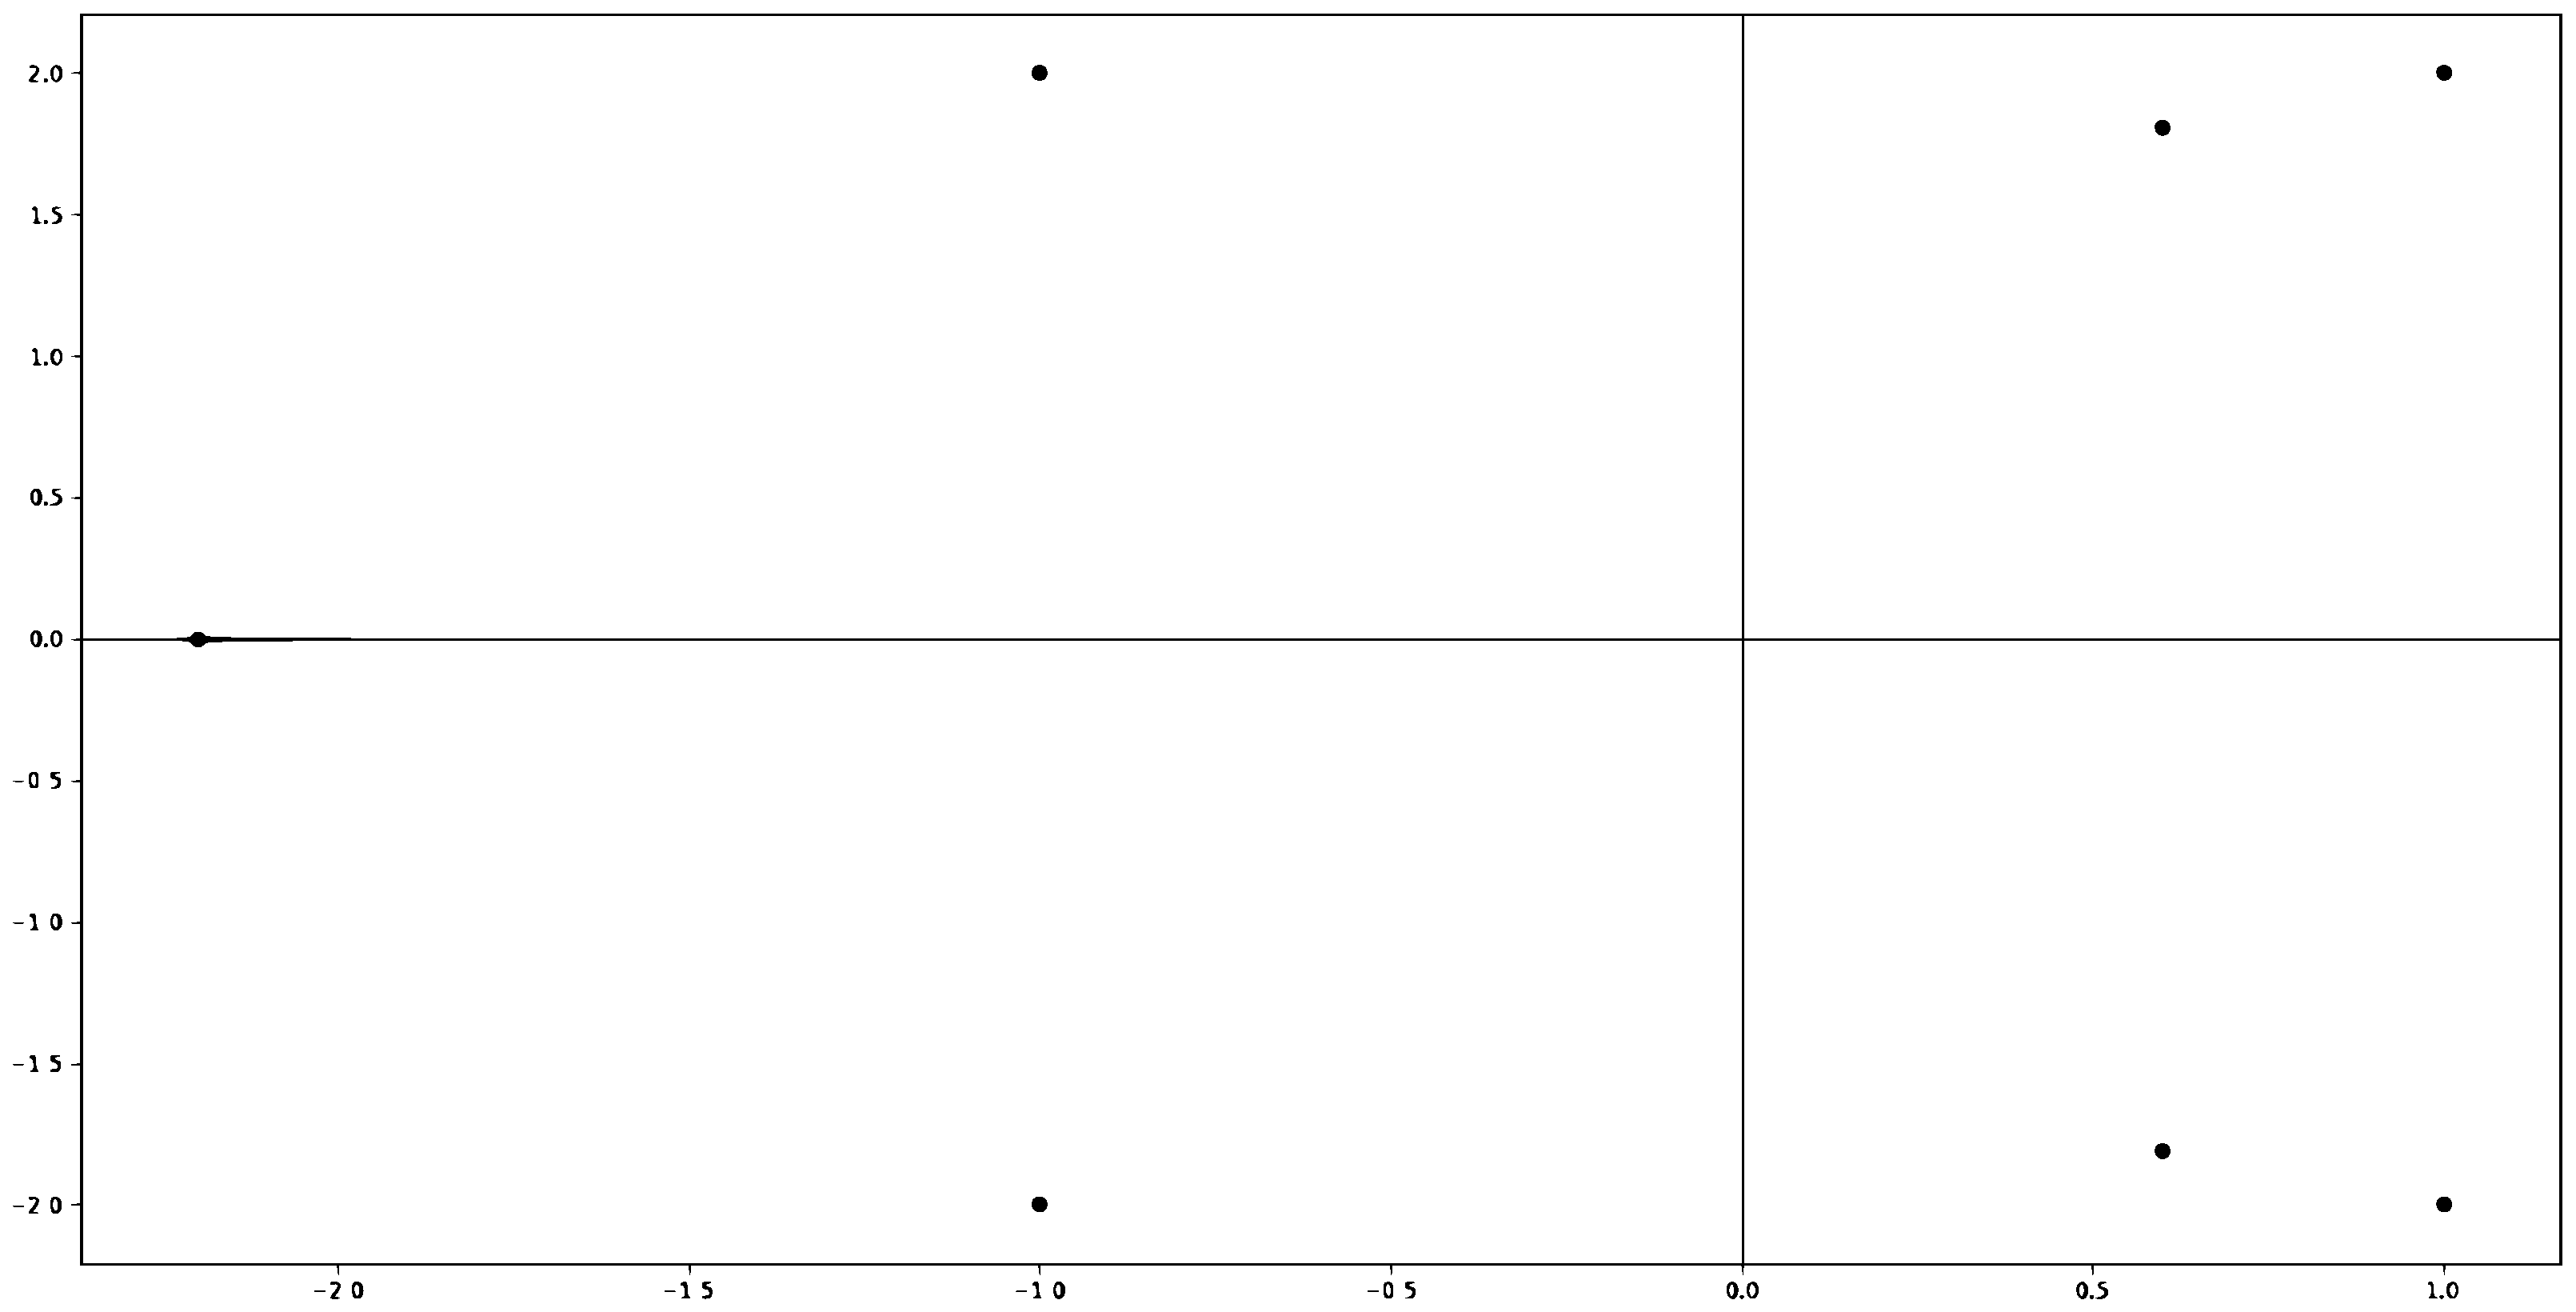
\includegraphics[scale=0.15]{figs/Roots.eps}
    
    \caption{Contour Plot Describing the values of given polynomial}
    \includegraphics[scale=0.15]{figs/f(z).png}
\end{figure}
